\documentclass[11pt,compress,t,notes=noshow, aspectratio=169, xcolor=table]{beamer}

\usepackage{../../style/lmu-lecture}
% Defines macros and environments
% This file is included in slides and exercises

% Rarely used fontstyle for R packages, used only in 
% - forests/slides-forests-benchmark.tex
% - exercises/single-exercises/methods_l_1.Rnw
% - slides/cart/attic/slides_extra_trees.Rnw
\newcommand{\pkg}[1]{{\fontseries{b}\selectfont #1}}

% Spacing helpers, used often (mostly in exercises for \dlz)
\newcommand{\lz}{\vspace{0.5cm}} % vertical space (used often in slides)
\newcommand{\dlz}{\vspace{1cm}}  % double vertical space (used often in exercises, never in slides)
\newcommand{\oneliner}[1] % Oneliner for important statements, used e.g. in iml, algods
{\begin{block}{}\begin{center}\begin{Large}#1\end{Large}\end{center}\end{block}}

% Don't know if this is used or needed, remove?
% textcolor that works in mathmode
% https://tex.stackexchange.com/a/261480
% Used e.g. in forests/slides-forests-bagging.tex
% [...] \textcolor{blue}{\tfrac{1}{M}\sum^M_{m} [...]
% \makeatletter
% \renewcommand*{\@textcolor}[3]{%
%   \protect\leavevmode
%   \begingroup
%     \color#1{#2}#3%
%   \endgroup
% }
% \makeatother


\title{Interpretable Machine Learning}
% \author{LMU}
%\institute{\href{https://compstat-lmu.github.io/lecture_iml/}{compstat-lmu.github.io/lecture\_iml}}
\date{}

\begin{document}

\newcommand{\titlefigure}{figure/feature-effect}
\newcommand{\learninggoals}{
%\item Intro to feature effects
\item ICE curves as local effect method
\item How to sample grid points for ICE curves
%\item Understand how to interpret ICE curves and PD plots
}

\lecturechapter{Individual Conditional Expectation (ICE) Plot}
\lecture{Interpretable Machine Learning}


\begin{frame}{Motivation}
%ICE curves show how different feature values of an observation affect its model prediction \newline $\Rightarrow$ \textbf{local interpretation method}
%From a local perspective, one might be interested in how changing feature values of an observation affect model prediction

\textbf{Question:} How does varying a single feature of an obs. affect its predicted outcome?

\smallskip

\textbf{Idea:} For a given observation, change the value of the feature of interest, and visualize how prediction changes

\smallskip

\textbf{Example:} On model prediction surface (left), select observation and visualize changes in prediction for different values of $x_2$, while keeping $x_1$ fixed \\ $\Rightarrow$ \textbf{local interpretation}

\bigskip
\centering
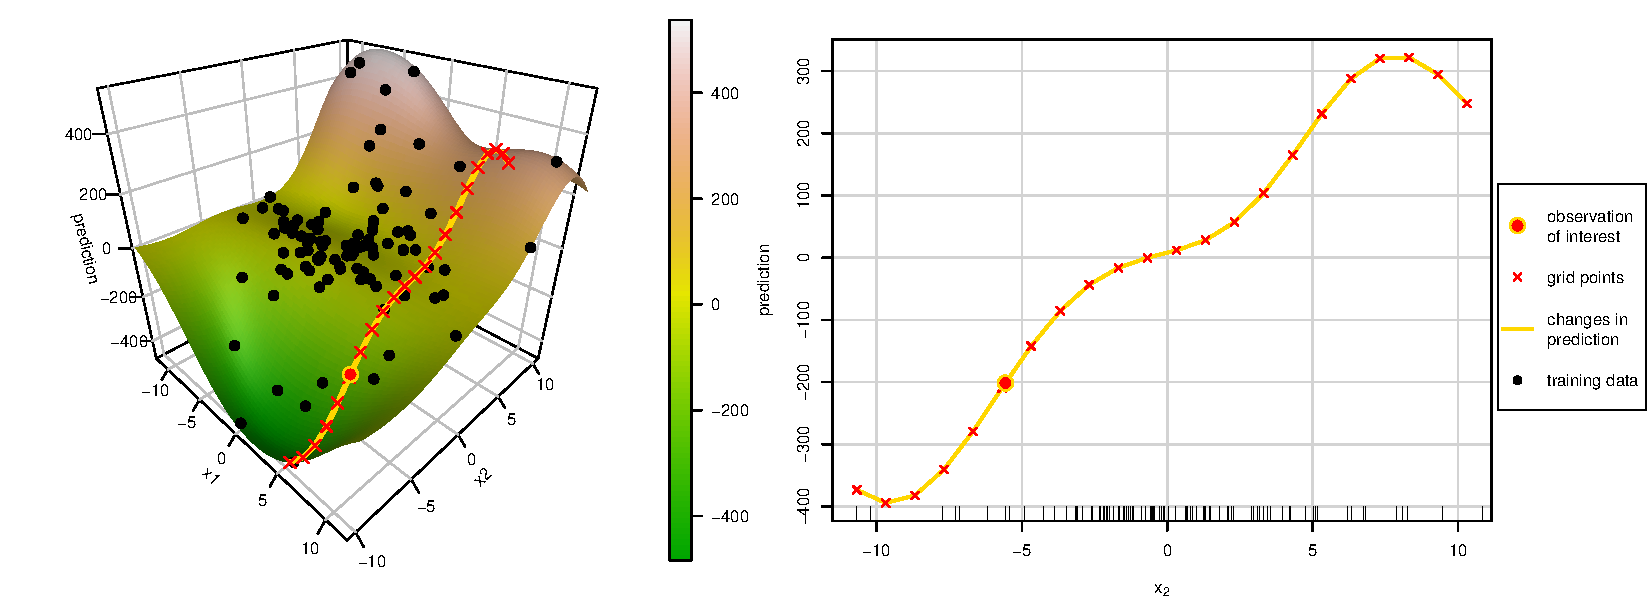
\includegraphics[width=\textwidth]{figure/ice_motivation}

%$\Rightarrow$ Repeat for all observations and average the curves for global feature effect ($\leadsto$ PD plots)
\end{frame}




\begin{frame}[c]{Individual Conditional Expectation (ICE) \citebutton{Goldstein et. al (2013)}{https://doi.org/10.1080/10618600.2014.907095}}

%Consider an index set $S \subseteq \{1, \dots, p\}$ and its complement $C = S^\complement$.
%\lz
\begin{columns}[T, totalwidth=\textwidth]
\begin{column}{0.16\textwidth} % 0.2 4.26cm
\includegraphics[page=1, trim=0cm 0.35cm 4.53cm 0.35cm, clip, width=0.9\textwidth]{../../figure_man/ice_plot_demo}
\end{column}
\begin{column}{0.84\textwidth}

%%%

%Assume each observation $\xi$ can be partitioned into $\xi_S$ and $\xi_C$ containing only feature values from the index set $S \subseteq \{1, \dots, p\}$ and its complement $C = S^\complement$, respectively.
%Assume each observation $\xi$ can be partitioned into $\xi_S$ and $\xi_C$ containing only feature values addressed by the feature's index set $S \subseteq \{1, \dots, p\}$ and its complement $C = S^\complement$, respectively.
%Assume each observation $\xi$ can be partitioned into $\xi_S$ and $\xi_C$ containing values from features addressed by the index set $S \subseteq \{1, \dots, p\}$ and its complement $C = S^\complement$, respectively.
Partition each observation $\xv$ into $\xv_S$ (feature(s) of interest) and $\xv_{-S}$ (remaining features)
\begin{itemize}
    \item[$\leadsto$] In practice, $\xv_S$ consists of one or two features \\ (i.e., $|S| \leq 2$ and ${-S} = S^\complement$).
    %, containing only feature values indexed by $S \subseteq \{1, \dots, p\}$ and its complement $C = S^\complement$.
\end{itemize}

\medskip

Formal definition of ICE curves: 
\begin{itemize}
    \item Define grid points $\xv_S^* = \xv_S^{*^{(1)}}, \dots, \xv_S^{*^{(g)}}$ to vary $\xv_S$
    \item Plot point pairs $ \Bigl\{\left(\xv_S^{*^{(k)}}, \fhice{S}^{(i)}(\xv_S^{*^{(k)}}) \right) \Bigr\}_{k=1}^g$
    \\where $\fhice{S}^{(i)}(\xv_S^*) = \fh(\xv_S^*, \xi_{-S})$
    \item For each $k$ connect point pairs to obtain \textbf{ICE curve}
\end{itemize}

\medskip

\begin{itemize}
    \item[$\leadsto$] ICE curves visualize how prediction of $i$-th observation changes after varying its feature values indexed by $S$ using grid points $\xv_S^*$ while keeping all values in $-S$ fixed
%by replacing the feature values $\xv_S^{(i)}$ with other values $\xv_S$ while keeping all other features in $\xi_C$ fixed:
%by varying the feature values in $\xv_S$ while keeping all other features in $\xi_C$ fixed.

% \begin{itemize}
%     \item[$\leadsto$] Plot \quad $\fh_{S}^{(i)}(\xv_S^*) \; \text{ vs. } \; \xv_S^*$ \\
%     where $\fh_{S}^{(i)}(\xv_S^*) = \fh(\xv_S^*, \xi_{-S})$ is prediction of $i$-th observation in which original feature value $\xi_S$ was replaced by $\xv_S^*$.
% \end{itemize}
\end{itemize}


%Visualize for \textbf{I}ndividual observations and \textbf{C}onditional on all other features how \textbf{E}xpected prediction changes

\end{column}
\end{columns}

% \begin{columns}[T, totalwidth=\textwidth]
% \begin{column}{0.6\textwidth}


% \end{column}
% \begin{column}{0.4\textwidth}
% %\begin{center}
% \centerline{\includegraphics[width=\textwidth]{figure_man/ice_bike10obs}}
% %\end{center}
% %\vspace{-0.3cm}
% \scriptsize{\textbf{Figure:} ICE Curves of 10 observations of the bike sharing dataset. Each line displays the change in prediction for a single observation due to varying the feature temperature.\par}
%
% \end{column}
% \end{columns}
%\footnote[frame]{Goldstein, A., Kapelner, A., Bleich, J., and Pitkin, E. (2013). Peeking Inside the Black Box: Visualizing Statistical Learning with Plots of Individual Conditional Expectation, 1-22. https://doi.org/10.1080/10618600.2014.907095}
\end{frame}

% \begin{frame}{Individual Conditional Expectation (ICE)}
%
% Steps to create an ICE curve of an observation regarding a single feature $\xv_S$ according to the \textbf{SIPA} framework:
%
% \begin{enumerate}
% \item \textbf{Sampling:} Choose grid points along $\xv_S$.
% \item For each grid point:
% \begin{itemize}
% \item \textbf{Intervention:} Replace the original feature value $\xv_S$ with the current grid value.
% \item \textbf{Prediction:} Get the model prediction with replaced feature value $\xv_S$.
% \end{itemize}
% \item \textbf{Aggregation:} none.
% \item \textbf{Visualization:} Draw a curve per observation with the grid points on the x-axis and the prediction on the y-axis.
% \end{enumerate}
%
% \footnote[frame]{Scholbeck, C. A., Molnar, C., Heumann, C., Bischl, B., and Casalicchio, G. (2019). Sampling, Intervention, Prediction, Aggregation: A Generalized Framework for Model Agnostic Interpretations. ECML PKDD 2019. (pp. 205-216).}
% \end{frame}

% \begin{frame}{Individual Conditional Expectation (ICE)}
%
% \begin{columns}[T, totalwidth=\textwidth]
% \begin{column}{0.4\textwidth}
% \includegraphics[page=1, trim=0cm 0.35cm 0.85cm 0.35cm, width=0.9\textwidth]{figure_man/ice_plot_demo}
% \end{column}
% \begin{column}{0.55\textwidth}
%
% \end{column}
% \end{columns}
% %\vspace*{\topsep}
%
% aa
% \end{frame}

\begin{frame}{ICE Curves - Illustration}

\begin{columns}[c, totalwidth=\textwidth]
\begin{column}{0.4\textwidth}
\includegraphics[page=2, trim=0cm 0.35cm 0.85cm 0.35cm, width=0.9\textwidth]{../../figure_man/ice_plot_demo}
\end{column}
\begin{column}{0.55\textwidth}

\end{column}
\end{columns}
\vspace*{\topsep}

\textbf{1. Step - Grid points:}

%For the $i$-th observation, we
\begin{itemize}
    \item Sample grid values $\xv_S^{*^{(1)}}, \dots, \xv_S^{*^{(g)}}$ along possible values of feature $S$ ($|S| = 1$)
\item For $\xv^{(i)} = (\xv_S, \xv_{-S})$, replace  $\xv_S$ with those grid values
\end{itemize}
%h observation with these sampled grid values.
%$\Rightarrow$ New artificial data points for $i$-th obs.
$\Rightarrow$ Creates new artificial points for $i$-th observation (here: $\xv_S^* = x_1^* \in \{1, 2, 3\}$ scalar)

\end{frame}

\begin{frame}{ICE Curves - Illustration}

\begin{columns}[c, totalwidth=\textwidth]
\begin{column}{0.4\textwidth}
\includegraphics<1>[page=3, trim=0cm 0.35cm 0.85cm 0.35cm, width=0.9\textwidth]{../../figure_man/ice_plot_demo}
\includegraphics<2>[page=4, trim=0cm 0.35cm 0.85cm 0.35cm, width=0.9\textwidth]{../../figure_man/ice_plot_demo}
\includegraphics<3>[page=5, trim=0cm 0.35cm 0.85cm 0.35cm, width=0.9\textwidth]{../../figure_man/ice_plot_demo}
\end{column}
\begin{column}{0.55\textwidth}
\includegraphics<1>[page=1, width=0.85\textwidth]{figure/ICE}
\includegraphics<2>[page=2, width=0.85\textwidth]{figure/ICE}
\includegraphics<3>[page=3, width=0.85\textwidth]{figure/ICE}
\end{column}
\end{columns}
\vspace*{\topsep}

\textbf{2. Step - Predict and visualize:}

For each artificially created data point of $i$-th observation, plot prediction $\fhice{S}^{(i)}(\xv_S^*)$ vs. grid values $\xv_S^*$:

$$\fhice{1}^{(i)}(x_1^*) = \fh(x_1^*, \xi_{2, 3}) \text{ vs. } x_1^* \in \{1, 2, 3\}$$

\end{frame}

% \begin{frame}{Individual Conditional Expectation (ICE)}

% \begin{columns}[T, totalwidth=\textwidth]
% \begin{column}{0.4\textwidth}
% \includegraphics[page=4, trim=0cm 0.35cm 0.85cm 0.35cm, width=0.9\textwidth]{figure_man/ice_plot_demo}
% \end{column}
% \begin{column}{0.55\textwidth}
% \includegraphics[page=2, width=0.85\textwidth]{figure/ICE}
% \end{column}
% \end{columns}
% \vspace*{\topsep}

% \textbf{Predict and visualize:}

% For each artificially created data point of $i$-th observation, plot prediction $\fh_{S}^{(i)}(\xv_S^*)$ vs. grid values $\xv_S^*$:

% $$\fh_{1}^{(i)}(x_1^*) = \fh(x_1^*, \xi_{2, 3}) \text{ vs. } x_1^* \in \{1, 2, 3\}$$
% \end{frame}

% \begin{frame}{Individual Conditional Expectation (ICE)}

% \begin{columns}[T, totalwidth=\textwidth]
% \begin{column}{0.4\textwidth}
% \includegraphics[page=5, trim=0cm 0.35cm 0.85cm 0.35cm, width=0.9\textwidth]{figure_man/ice_plot_demo}
% \end{column}
% \begin{column}{0.55\textwidth}
% \includegraphics[page=3, width=0.85\textwidth]{figure/ICE}
% \end{column}
% \end{columns}
% \vspace*{\topsep}

% \textbf{Predict and visualize:}

% For each artificially created data point of $i$-th observation, plot prediction $\fh_{S}^{(i)}(\xv_S^*)$ vs. grid values $\xv_S^*$:

% $$\fh_{1}^{(i)}(x_1^*) = \fh(x_1^*, \xi_{2, 3}) \text{ vs. } x_1^* \in \{1, 2, 3\}$$
% \end{frame}

% \begin{frame}{Individual Conditional Expectation (ICE)}

% % \begin{columns}[T]
% % \begin{column}{0.4\textwidth}
% % \includegraphics[page=5, trim=0cm 0.35cm 0.85cm 0.35cm, width=0.9\textwidth]{figure_man/ice_plot_demo}
% % \end{column}
% % \begin{column}{0.55\textwidth}
% % \includegraphics[page=3, width=0.85\textwidth]{figure/ICE}
% % \end{column}
% % \end{columns}
% % \vspace*{\topsep}

% \begin{itemize}
%     \item \textbf{Interpretation:} \textbf{ICE} curve visualizes for \textbf{I}ndividual observations and \textbf{C}onditional on all other features (by keeping all other features constant) how \textbf{E}xpected prediction changes
%     \item
%     \item For global view, repeat procedure for all observations
% \end{itemize}

% % \textbf{Definition:}

% % ICE curves involve plotting the pairs $ \{(\xv_S^{*^{(k)}}, \fh_{S}^{(i)}(\xv_S^*{^{(k)}})) \}_{k=1}^g $ for grid points $\xv_S^{*^{(1)}}, \dots, \xv_S^{*^{(g)}}$.
% \end{frame}

\begin{frame}{ICE Curves - Illustration}

\begin{columns}[T, totalwidth=\textwidth]
\begin{column}{0.4\textwidth}
\includegraphics<1>[page=6, trim=0cm 0.35cm 0.85cm 0.35cm, width=0.9\textwidth]{../../figure_man/ice_plot_demo}
\includegraphics<2>[page=7, trim=0cm 0.35cm 0.85cm 0.35cm, width=0.9\textwidth]{../../figure_man/ice_plot_demo}
\end{column}
\begin{column}{0.55\textwidth}
\includegraphics<1>[page=4, width=0.85\textwidth]{figure/ICE}
\includegraphics<2>[page=5, width=0.85\textwidth]{figure/ICE}
\end{column}
\end{columns}
\vspace*{\topsep}

\textbf{3. Step - Repeat for other observations:}

ICE curve for\only<1>{ $i=2$ }\only<2>{ $i=3$ }connects all predictions at grid values associated to $i$-th obs.
\end{frame}

% \begin{frame}{ICE Curves - Illustration}

% \begin{columns}[T, totalwidth=\textwidth]
% \begin{column}{0.4\textwidth}
% \includegraphics[page=7, trim=0cm 0.35cm 0.85cm 0.35cm, width=0.9\textwidth]{figure_man/ice_plot_demo}
% \end{column}
% \begin{column}{0.55\textwidth}
% %\begin{center}
% \includegraphics[page=5, width=0.85\textwidth]{figure/ICE}
% %\end{center}
% \end{column}
% \end{columns}
% \vspace*{\topsep}

% \textbf{3. Step - Repeat for other observations:}

% ICE curve for $i=3$ connects all predictions at grid values associated to $i$-th obs.
% %The ICE curve of observation $i=3$ connects all predictions at the corresponding grid values associated to the $i$-th obs.

% % \textbf{Definition:}

% % ICE curves involve plotting the pairs $ \{(\xv_S^{*^{(k)}}, \fh_{S}^{(i)}(\xv_S^*{^{(k)}})) \}_{k=1}^g $ for grid points $\xv_S^{*^{(1)}}, \dots, \xv_S^{*^{(g)}}$.
% \end{frame}

\begin{frame}{ICE Curves - Interpretation}
\textbf{Example:} Prediction surface of a model (left), select observation and visualize changes in prediction for different values of $x_2$ while keeping $x_1$ fixed \\ $\Rightarrow$ \textbf{local interpretation}

\bigskip
\centering
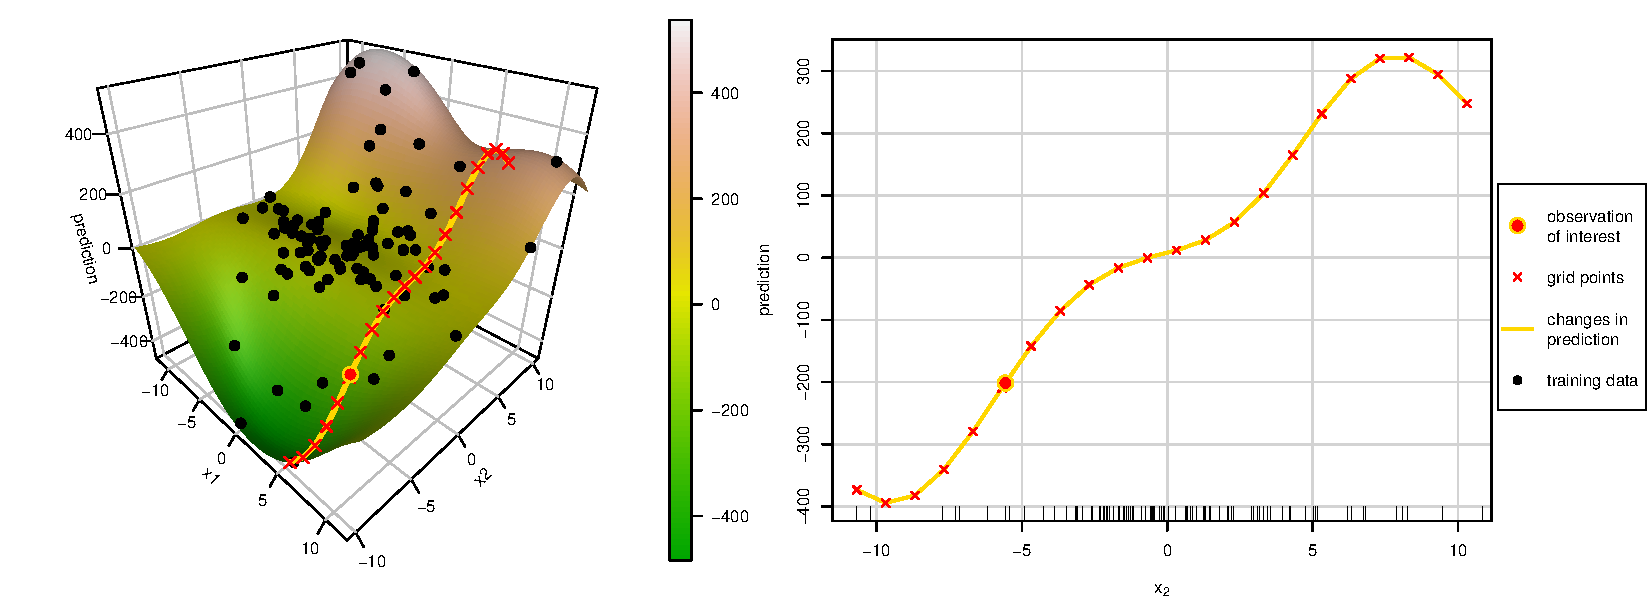
\includegraphics[width=\textwidth]{figure/ice_motivation}

%% Wie nutzt man ICE Kurven zur lokalen Interpretation?
\end{frame}


\begin{frame}{Comments on Grid values}
\begin{itemize}
%\item ICE curves show how different feature values of an observation affect its prediction \newline $\Rightarrow$ \textbf{local interpretation method}
\item Plotting ICE curves involves generating grid values $\xv_S^*$; visualized on x-axis
\item Common choices for grid values are
\begin{itemize}
\item equidistant grid values within feature range
\item randomly sampled values of observed feature values
\item quantile values of observed feature values
\end{itemize}
\item Except equidistant grid, the other two options preserve (approximately) the marginal distribution of feature of interest
%$\Rightarrow$ Avoids unrealistic feature values for distributions with outliers %or dependencies
\item<2> Correlations/interactions $\leadsto$ unrealistic values in all three methods
%(to be addressed with ALE plots later)%Preferable for skewed distributions (with outliers) to avoid using unrealistic feature values.
% \begin{itemize}
% \item equidistant grid values:
% \item sub-sampled grid values:
% \item quantile grid values:
% \end{itemize}
\end{itemize}

\vspace{0.3cm}
\centering
\includegraphics<1>[width=0.85\textwidth, trim=0cm 0cm 0cm 0cm, clip]{figure/sampling2}
\includegraphics<2>[width=0.85\textwidth, trim=0cm 0cm 0cm 0cm, clip]{figure/sampling}


\end{frame}

% bike sharing example + defaults
% \begin{frame}{ICE curves example and practical considerations}

% \begin{columns}[T]
% \begin{column}{0.55\textwidth}
% \small
% \begin{itemize}
%   \item \textbf{Grid points}  
%         \begin{itemize}
%             \item Too few $\Rightarrow$ misses sharp changes%
%             \item Too many $\Rightarrow$ time intensive%
%         \end{itemize}
%   \item \textbf{ICE curves}  
%         \begin{itemize}
%             \item Too few $\Rightarrow$ heterogeneity is hidden%
%             \item Too many $\Rightarrow$ plot cluttered, time intensive%
%         \end{itemize}
%   \item Default values for popular libraries: 
% \end{itemize}

% \vspace{1em}
% \centering
% \begin{tabular}{lccc}
% \textbf{Library} & \textbf{Language} & \textbf{Grid points} & \textbf{ICE curves}\\\hline
% scikit--learn & Py & 100 & 1\,000\\
% PDPbox        & Py & 10  & num. rows\\
% iml           & R  & 20  & num. rows\\
% pdp           & R  & 51  & num. rows\\
% \end{tabular}
% \end{column}

% % -------- RIGHT COLUMN: FIGURE --------
% \begin{column}{0.45\textwidth}
% \centering
% 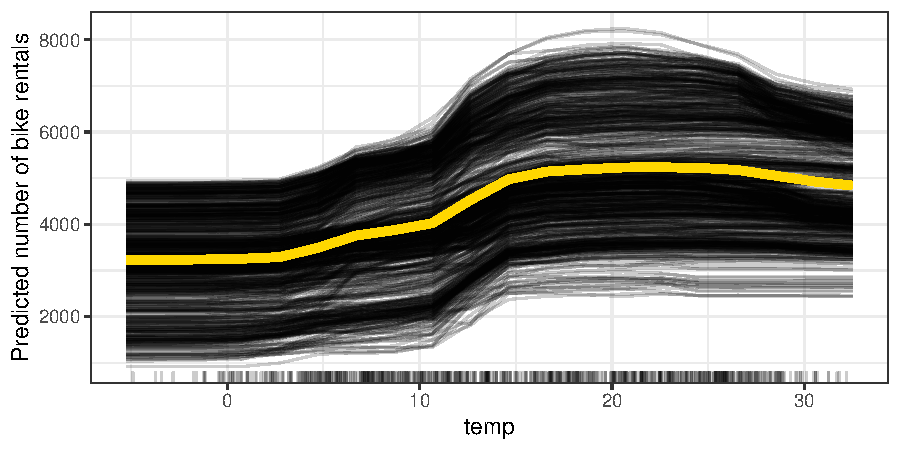
\includegraphics[width=\textwidth]{figure/pdp_bike.pdf}

% \vspace{0.7em}
% \scriptsize
% The \textbf{black curves} are the ICE curves and he \textbf{yellow line} is the "average ICE curve". It is called a Partial dependence plot and will be discussed in the next slide set.
% \end{column}
% \end{columns}

% \end{frame}

\endlecture
\end{document}
